\documentclass{article}
\usepackage{neurips_2026}
\usepackage[utf8]{inputenc} % allow utf-8 input
\usepackage[T1]{fontenc}    % use 8-bit T1 fonts
\usepackage{amsmath,amssymb,mathtools,amsthm}
\usepackage{hyperref}       % hyperlinks
\usepackage{url}            % simple URL typesetting
\usepackage{graphicx}       % figures
\usepackage{booktabs}       % professional-quality tables
\usepackage{amsfonts}       % blackboard math symbols
\usepackage{nicefrac}       % compact symbols for 1/2, etc.
\usepackage{microtype}      % microtypography
\usepackage{xcolor}         % colors

\usepackage[most]{tcolorbox}
\usepackage{algorithm}
\usepackage{enumitem}
\usepackage{algorithm}
\usepackage{algpseudocode}
\usepackage{tabularx}
\usepackage{array}
\usepackage{xspace}

\newcolumntype{L}[1]{>{\raggedright\arraybackslash}p{#1}}


\let\REQUIRE\Require
\let\ENSURE\Ensure
\let\STATE\State
\let\FOR\For
\let\ENDFOR\EndFor
\let\IF\If
\let\ENDIF\EndIf
\let\RETURN\Return
\usepackage[capitalize,noabbrev]{cleveref}
\usepackage{subcaption}


\title{Your Drift Deserves Better Support}


\author{%
  David S.~Hippocampus \\
  Department of Computer Science\\
  Cranberry-Lemon University\\
  Pittsburgh, PA 15213 \\
  \texttt{hippo@cs.cranberry-lemon.edu} \\
  % examples of more authors
  % \And
  % Coauthor \\
  % Affiliation \\
  % Address \\
  % \texttt{email} \\
  % \AND
  % Coauthor \\
  % Affiliation \\
  % Address \\
  % \texttt{email} \\
  % \And
  % Coauthor \\
  % Affiliation \\
  % Address \\
  % \texttt{email} \\
}


% Soft ML-paper colors.
\definecolor{mlblue}{HTML}{4C78A8}
\definecolor{mlorange}{HTML}{F58518}
\definecolor{mlgreen}{HTML}{54A24B}
\definecolor{mlpurple}{HTML}{B279A2}
\definecolor{mlgray}{HTML}{6B7280}

\newtcolorbox{contributionbox}[1]{
  enhanced,
  breakable,
  colback=#1!7,
  colframe=#1!42!black,
  boxrule=0.45pt,
  arc=2pt,
  left=6pt,
  right=6pt,
  top=5pt,
  bottom=5pt,
  before skip=0.75em,
  after skip=1.6em
}

\newcommand{\introparagraph}[1]{%
  \par\noindent\textbf{#1.}\quad%
}

\newcommand{\placeholderbox}[2]{
\begin{center}
\fbox{
\begin{minipage}[c][#1][c]{0.92\linewidth}
\centering
\textcolor{mlgray}{#2}
\end{minipage}
}
\end{center}
}

\newcommand{\F}{\mathbf{F}}
\newcommand{\V}{\mathbf{V}}
\newcommand{\x}{\mathbf{x}}
\newcommand{\y}{\mathbf{y}}
\newcommand{\yp}{\mathbf{y}^{+}}
\newcommand{\yn}{\mathbf{y}^{-}}
\newcommand{\z}{\mathbf{z}}
\newcommand{\sg}{\operatorname{sg}}
\newcommand{\softmax}{\operatorname{softmax}}
\newcommand{\Apos}{A^{+}}
\newcommand{\Aneg}{A^{-}}
\newcommand{\dms}{d_{\mathrm{MS}}}
\newcommand{\deuc}{d_{\mathrm{Euc}}}
\newcommand{\sep}{\mathrm{sep}}
\newcommand{\coup}{\mathrm{coup}}



\newcommand{\model}{\textsc{SupportDrift}\xspace}
\newcommand{\base}{\textsc{Drift-Base}\xspace}
\newcommand{\R}{\mathbb{R}}
\newcommand{\E}{\mathbb{E}}
\newcommand{\TopK}{\operatorname{TopK}}
\newcommand{\FID}{\mathrm{FID}}
\newcommand{\IS}{\mathrm{IS}}
\newcommand{\todoresult}[1]{\textcolor{gray}{[#1]}}

\newcommand{\Pset}{\mathcal{P}}
\newcommand{\Nset}{\mathcal{N}}
\newcommand{\Bpos}{\mathcal{B}^{+}}
\newcommand{\Bneg}{\mathcal{B}^{-}}



\begin{document}


\maketitle


% ============================================================
% Abstract
% ============================================================

\begin{abstract}
% Drifting models train one-step generators by moving generated samples along a data-dependent drift field.
% While the population drifting field is well-motivated, the object used during training is a finite-support estimator built from sampled positives, sampled negatives, a similarity function, and affinity weights.
% We show that this estimator is a central bottleneck.
% The original estimator suffers from three measurable pathologies: uniform positives can produce diffuse attraction, Euclidean feature distances can retrieve false neighbors, and coupled positive--negative affinities can attenuate the update through cross-side softmax mass.
% We propose a support-aware drift estimator that repairs these failures with positive-enhanced sampling, a structure-aware support geometry, and side-separated affinity normalization.
% Our diagnostics isolate the corresponding estimator improvements, and compute-matched ImageNet experiments test whether these repairs translate into improved one-step generation.
% Our results recast Drifting Models as an estimator-design problem: the drift field is only as useful as the finite supports used to approximate it.
Drifting models train one-step generators by moving generated samples along a vector field estimated from positive data supports and negative generated supports.
The original framework defines this field as a population object, but practical training uses a small, finite support set at every update.
In this paper, we show that this finite-support estimator is a central bottleneck.
It fails in three measurable ways: First, uniform same-class positives produce diffuse and weakly aligned attraction. Second, Euclidean feature distance retrieves false neighbors under controlled local-structure tests. Third, coupled positive/negative affinities suppress updates through a cross-side product gate.
We turn these observations into a drop-in estimator, \model, which improves the support distribution, its geometry, and the side-specific normalization of the drift field.
Across ImageNet-256 experiments, \model improves early convergence from \todoresult{baseline FID@20k} to \todoresult{ours FID@20k}, reaches \todoresult{final FID}, and preserves native one-step inference.
Beyond aggregate FID/IS, our analyses show that the proposed estimator produces more local positive forces, fewer false neighbors, and less cross-side attenuation.

\end{abstract}

% ============================================================
% Introduction
% ============================================================

\section{Introduction}
\label{sec:introduction}

Generative modeling is often made tractable by spreading computation across many inference steps.
Diffusion and flow-based models implement this principle explicitly: generation proceeds through a sequence of small transformations that gradually move a simple prior toward the data distribution.
Drifting Models offer a different tradeoff.
They perform generation with a single network evaluation, but use training itself to evolve the pushforward distribution toward the data distribution.
At each training step, generated samples are moved by a data-dependent drifting field; when the generated and data distributions match, this field vanishes.

A population-level view is elegant.
However, the object used during training is not the population drifting field.
It is a finite-support estimator built from sampled positives, sampled negatives, a similarity function, and affinity weights.
Thus, practical drifting is not determined only by the definition of the population field.
It is determined by the quality of the stochastic estimator that approximates this field at every optimization step.

The original implementation makes natural choices for this estimator.
Positive supports are sampled uniformly from same-class data.
Similarity is measured by Euclidean distance in feature space.
Positive and negative supports are normalized through coupled affinities.
These choices are simple and effective, but they also encode strong assumptions:
same-class positives are assumed to provide local attraction, Euclidean distance is assumed to retrieve useful drift targets, and coupled normalization is assumed to preserve a stable attraction--repulsion update.
We show that these assumptions fail in measurable ways.

This motivates the central question of this paper:
\begin{center}
\emph{What makes a finite-support drift estimator reliable?}
\end{center}

We answer this question by treating support selection, support geometry, and support weighting as primary components of the model.
Rather than introducing modifications only through final sample quality, we diagnose concrete estimator failure modes and resolve them step-by-step.

\introparagraph{Diffuse positive supports}
Uniform same-class sampling often yields a high-entropy positive affinity distribution.
Many positives technically contribute, but few are locally relevant to each generated anchor sample.
The resulting attraction can average over unrelated same-class modes, producing a weak or poorly aligned positive force.
We measure this using positive-affinity entropy, top-$k$ mass, force norm, and cosine alignment with a large-pool nearest-neighbor oracle force.

\begin{contributionbox}{mlblue}
\textbf{Contribution 1: Positive supports should be local, not merely same-class.}
We show that naïve uniform positive sampling can produce diffuse attraction, and we introduce positive-enhanced sampling, which mixes nearest positive supports with random positives to improve local force alignment while preserving coverage.
\end{contributionbox}

\introparagraph{False neighbors under Euclidean geometry}
The second failure is caused by the support geometry.
Euclidean distance in the baseline feature space can retrieve same-class supports that are close in global feature magnitude but poor as drift targets.
To test this without human annotation, we construct controlled ranking tasks in which each anchor is compared against a weak positive view, a spatially corrupted view, and same-label decoys.
A useful metric should rank the weak view highly and assign a positive margin against the corrupted view.

\begin{contributionbox}{mlorange}
\textbf{Contribution 2: Drift supports require a structure-aware geometry.}
We show that Euclidean distance induces measurable false-neighbor errors, and we replace it with a structure-aware distance that better respects local statistics and controlled spatial corruptions.
\end{contributionbox}

\introparagraph{Cross-side attenuation from coupled affinities}
The third failure is caused by the coefficient rule.
In a simplified row-softmax form of the original estimator, positive and negative supports share a joint normalization.
If $\Apos$ and $\Aneg$ denote the total joint-softmax mass assigned to the positive and negative sides, then the coupled update behaves approximately as
\begin{equation}
\F_{\coup}
\approx
\Apos \Aneg
\left(
\bar{\F}^{+}
+
\bar{\F}^{-}
\right),
\label{eq:intro_product_gate}
\end{equation}
where $\bar{\F}^{+}$ and $\bar{\F}^{-}$ are side-normalized attraction and repulsion forces.
Thus, the original rule gates the entire update by a product of cross-side evidence.
When one side dominates the joint softmax, the other side is suppressed, and the drift magnitude can collapse even though both supports were deliberately sampled.

\begin{contributionbox}{mlgreen}
\textbf{Contribution 3: Positive and negative evidence should not gate each other.}
We identify cross-side attenuation as a failure mode of coupled affinities and propose side-separated affinity normalization, which preserves attraction and repulsion as independently normalized forces.
\end{contributionbox}

These three observations suggest a different view of drifting models.
The main bottleneck is not only the design of the population field, but the reliability of its finite-support estimator.
We therefore propose a support-aware drift estimator that combines positive-enhanced sampling, structure-aware similarity, and side-separated weights.
The resulting method changes neither the one-step generator nor the basic training paradigm; it changes the quality of the training signal.

We validate this view in two stages.
First, we use offline diagnostics on fixed generator checkpoints to isolate estimator behavior without retraining.
These probes test whether each proposed change repairs the failure mode it is meant to address.
Second, we train ImageNet generators under compute-matched settings.
Across pilots, improving the support estimator improves early convergence and sample quality under the same backbone, optimizer, and training budget.

\begin{contributionbox}{mlpurple}
\textbf{Contribution 4: A better finite-support estimator improves one-step generation.}
On ImageNet, estimator-level repairs translate into improved generative performance under compute-matched training, showing that the proposed diagnostics predict practically useful changes rather than only post-hoc explanations.
\end{contributionbox}

Overall, our results recast Drifting Models as an estimator-design problem.
The original framework specifies a compelling population drift.
Our work shows that the finite supports used to approximate this drift deserve equal attention.
Better supports, better geometry, and better side-specific weighting produce a more reliable drift signal before any aggregate sample-quality metric is considered.

% ============================================================
% Finite-support reframing
% ============================================================

\section{Drifting as Finite-Support Estimation}
\label{sec:finite_support}

Drifting Models define a training-time vector field that moves generated samples toward the data distribution.
Let $p$ denote the data distribution and let $q_\theta = (f_\theta)_\# p_\epsilon$ denote the pushforward distribution of the generator.
For a generated sample $\x \sim q_\theta$, the population drifting field can be written as an attraction--repulsion field
\begin{equation}
\V_{p,q_\theta}(\x)
=
\V^{+}_{p}(\x)
-
\V^{-}_{q_\theta}(\x),
\label{eq:population_drift}
\end{equation}
where the positive field attracts $\x$ toward data samples and the negative field repels it from generated samples.
When $p=q_\theta$, the two sides cancel under the anti-symmetry condition of the original framework, yielding a zero-drift equilibrium.

In practice, the population field in \cref{eq:population_drift} is not available.
Training uses finite supports.
For each anchor $\x$, we draw positive supports $S^+=\{\yp_j\}_{j=1}^{M_+}$ from the data distribution and negative supports $S^-=\{\yn_k\}_{k=1}^{M_-}$ from the generated distribution.
The implemented update is therefore a stochastic estimator of the form
\begin{equation}
\widehat{\V}(\x;S^+,S^-,d,w)
=
\sum_{j=1}^{M_+}
w_j^+(\x,S^+,S^-)
(\yp_j-\x)
-
\sum_{k=1}^{M_-}
w_k^-(\x,S^+,S^-)
(\yn_k-\x).
\label{eq:finite_support_estimator}
\end{equation}
This expression makes explicit that finite-support drifting has three estimator components:
the sampled supports $S^+$ and $S^-$, the distance or similarity function $d$, and the coefficient rule $w$.

The original estimator uses simple defaults for these components.
Positive and negative supports are sampled uniformly from their respective pools.
Distances are Euclidean in the chosen feature space.
Affinity weights are computed from temperature-scaled distances, with positive and negative supports coupled through the normalization.
These choices give a simple estimator, but not necessarily a reliable one.
The remainder of the paper studies the failure modes induced by these defaults and introduces a support-aware replacement.

% ============================================================
% Estimator pathologies
% ============================================================

\section{Three Pathologies of the Original Estimator}
\label{sec:pathologies}

The finite-support view in \cref{eq:finite_support_estimator} suggests that estimator quality can fail for distinct reasons.
The supports may be uninformative, the geometry may retrieve poor neighbors, or the coefficient rule may distort the force.
We isolate these three failure modes with diagnostics that do not require human annotation and can be run offline on fixed generator checkpoints.

\subsection{Uniform positives produce diffuse attraction}
\label{subsec:diffuse_positives}

The original estimator treats uniformly sampled same-class positives as a local approximation to the data distribution around a generated anchor.
This assumption is weak on ImageNet.
A class can contain many visual modes, and a uniformly sampled same-class positive set may contain few samples that are locally relevant to a particular anchor.

For an anchor $\x$ and positive supports $S^+=\{\yp_j\}_{j=1}^{M}$, define positive affinities
\begin{equation}
a_j^{+}(R)
=
\frac{\exp(-d(\x,\yp_j)/R)}
{\sum_{\ell=1}^{M}\exp(-d(\x,\yp_\ell)/R)}.
\label{eq:positive_affinity}
\end{equation}
The induced positive force is
\begin{equation}
\F^{+}(\x)
=
\sum_{j=1}^{M}
a_j^{+}(R)(\yp_j-\x).
\label{eq:positive_force}
\end{equation}
A diffuse positive kernel has high entropy, low top-$k$ mass, and a force direction that may average over unrelated same-class modes.

We evaluate this failure mode by comparing two positive samplers at the same budget:
uniform positives and positive-enhanced positives.
For each anchor, we measure normalized entropy $H(a^+)/\log M$, effective support fraction $\exp(H(a^+))/M$, top-$1$ and top-$5$ affinity mass, positive-force norm, and alignment with a large-pool oracle force.
The oracle force is computed from the nearest positives inside a larger candidate pool:
\begin{equation}
\F^{*}_{\mathrm{pos}}(\x)
=
\sum_{j\in\operatorname{Top64}(\x)}
a_j^{*}(\yp_j-\x).
\label{eq:oracle_positive_force}
\end{equation}
The relevant diagnostic is not entropy alone.
A useful positive sampler should produce a more concentrated positive kernel and improve cosine alignment with $\F^{*}_{\mathrm{pos}}$.

\begin{figure}[h!]
\centering
\placeholderbox{0.23\textheight}{
Positive-sampling diagnostic panel.\\
Paired plots over anchors: normalized entropy, top-5 mass, oracle-force cosine.\\
Compare uniform positives vs positive-enhanced positives at equal support budget.
}
\caption{
\textbf{Uniform positives produce diffuse attraction.}
Positive-enhanced sampling should reduce positive-kernel diffusion and improve alignment with a large-pool local positive force.
}
\label{fig:positive_sampling_probe}
\end{figure}

\begin{table}[h!]
\centering
\caption{
\textbf{Positive-support diagnostic summary.}
Report medians and interquartile ranges over anchors.
}
\label{tab:positive_sampling_summary}
\begin{tabular}{lrrrr}
\toprule
Sampler & Entropy $\downarrow$ & Top-5 mass $\uparrow$ & $\|\F^{+}\|$ & Oracle cosine $\uparrow$ \\
\midrule
Uniform positives & -- & -- & -- & -- \\
Positive-enhanced & -- & -- & -- & -- \\
\bottomrule
\end{tabular}
\end{table}

\subsection{Euclidean distance retrieves false neighbors}
\label{subsec:false_neighbors}

The second estimator component is the support geometry.
The baseline uses Euclidean distance in feature space.
This assumes that Euclidean nearest neighbors are useful drift targets.
However, feature-space magnitude and local visual structure need not agree.
A support can be close under Euclidean distance while being a poor local correction for the generated anchor.

We test this with a controlled ranking task.
For each anchor image or feature $\x$, we construct a candidate set containing a weak positive view $\x_{\mathrm{weak}}$, a spatially corrupted view $\x_{\mathrm{bad}}$, and a bank of geometric impostors mined by Euclidean distance.
For each metric $d_m$, we compute the rank of the weak view and the corruption margin
\begin{equation}
\Delta_m
=
d_m(\x,\x_{\mathrm{bad}})
-
d_m(\x,\x_{\mathrm{weak}}).
\label{eq:corruption_margin}
\end{equation}
A reliable support geometry should rank $\x_{\mathrm{weak}}$ above both spatial corruptions and mined geometric impostors.

This diagnostic separates metric quality from subjective nearest-neighbor inspection.
We also evaluate a generated-anchor stress matrix whose desired behavior is visually unambiguous: a weak view should stay close, while roll, patch-shuffle, and Euclidean-mined layout impostors should move far away.
The quantitative object is the retrieval behavior of the metric; the visual panel only explains the controlled transformations.

\begin{figure}[h!]
\centering
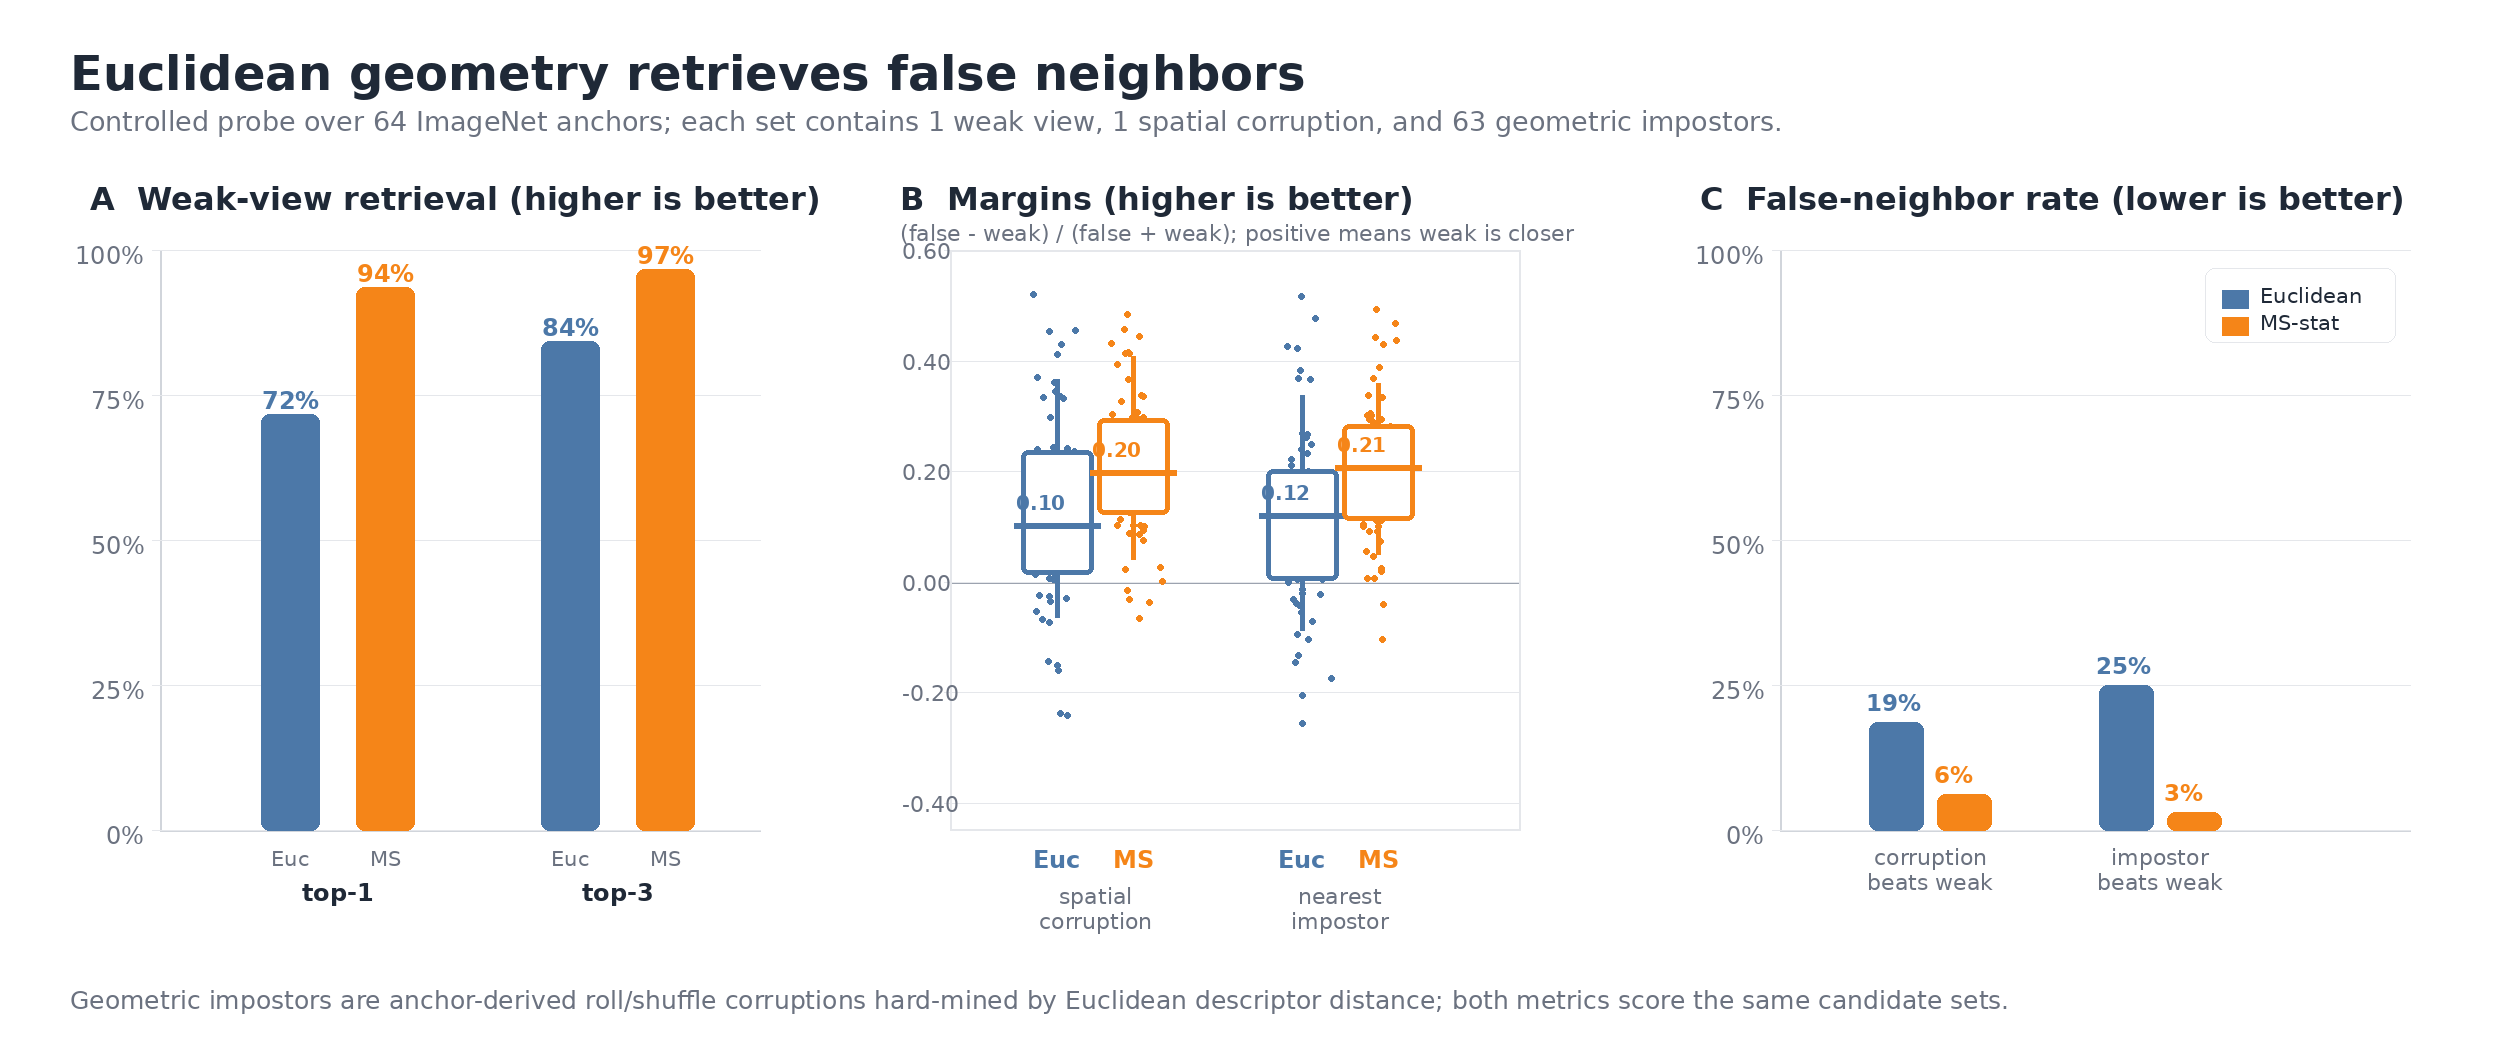
\includegraphics[width=\linewidth]{figures/euclidean_false_neighbors.png}
\caption{
\textbf{Euclidean geometry retrieves false neighbors.}
In a harder controlled probe over 64 ImageNet anchors with 63 Euclidean-mined geometric impostors per anchor, Euclidean feature geometry ranks the weak view first/top-3 for 71.9\%/84.4\% of anchors.
The proposed multiscale-statistics geometry improves this to 93.8\%/96.9\%, while reducing corruption and impostor false-neighbor errors from 18.8\%/25.0\% to 6.2\%/3.1\%.
}
\label{fig:similarity_probe}
\end{figure}

\begin{figure}[h!]
\centering
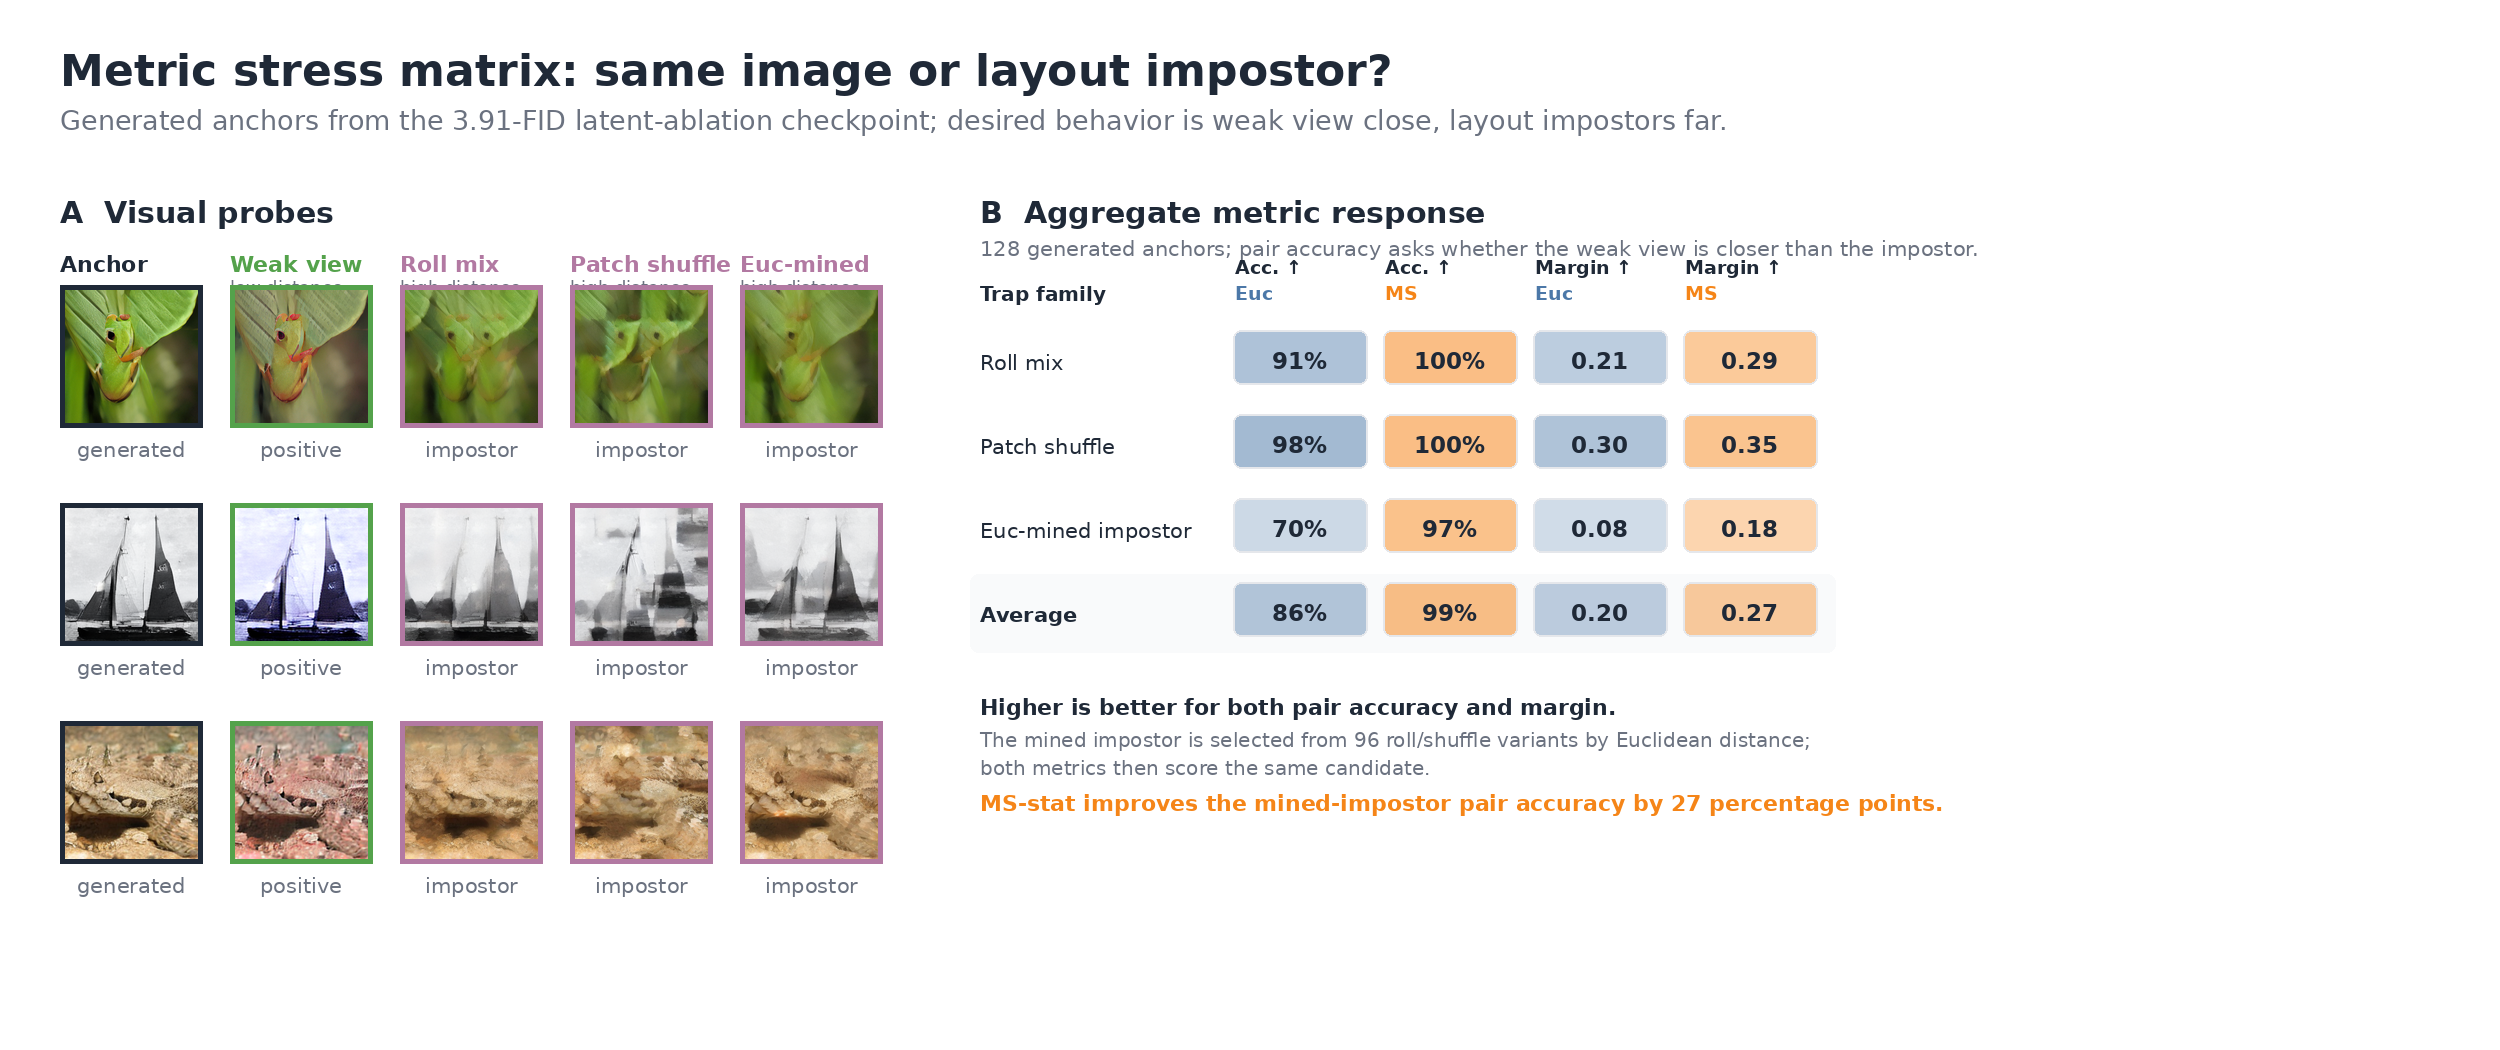
\includegraphics[width=\linewidth]{figures/metric_stress_matrix.png}
\caption{
\textbf{Metric stress matrix.}
Rows visualize generated anchors from the 3.91-FID latent-ablation checkpoint, their weak positive views, and layout-breaking impostors.
Over 128 generated anchors, Euclidean distance handles simple roll/patch corruptions reasonably but drops to 70.3\% pair accuracy on Euclidean-mined impostors.
The proposed multiscale-statistics metric reaches 96.9\% on the mined-impostor trap and improves average pair accuracy across traps from 86.5\% to 99.0\%.
}
\label{fig:metric_stress_matrix}
\end{figure}

\subsection{Coupled affinities attenuate the update}
\label{subsec:cross_side_attenuation}

The third estimator component is the coefficient rule.
In the coupled estimator, positive and negative supports are normalized together.
This creates cross-side dependence: the mass assigned to one side affects the contribution of the other.

Consider a simplified row-softmax version of the coupled rule.
Let $a_j^+$ and $a_k^-$ be the joint-softmax weights assigned to positive and negative supports, and define the total side masses
\begin{equation}
\Apos = \sum_j a_j^+,
\qquad
\Aneg = \sum_k a_k^-.
\label{eq:side_masses}
\end{equation}
The side-normalized forces are
\begin{equation}
\bar{\F}^{+}
=
\sum_j
\frac{a_j^+}{\Apos}
(\yp_j-\x),
\qquad
\bar{\F}^{-}
=
-
\sum_k
\frac{a_k^-}{\Aneg}
(\yn_k-\x).
\label{eq:side_normalized_forces}
\end{equation}
Under the coupled product form, the update is approximately
\begin{equation}
\F_{\coup}
\approx
\Apos\Aneg
\left(
\bar{\F}^{+}
+
\bar{\F}^{-}
\right).
\label{eq:coupled_product_gate}
\end{equation}
Thus, coupled affinities behave like a product-of-evidence gate.
The drift magnitude becomes small whenever either side receives little joint-softmax mass.
This can happen even when both supports are present, because low mass may simply mean that the other side contains a harder neighbor.

We measure this effect on real drift batches by comparing the coupled update with the side-separated update
\begin{equation}
\F_{\sep}
=
\bar{\F}^{+}
+
\bar{\F}^{-}.
\label{eq:separate_force}
\end{equation}
For each anchor, we log the norm ratio
\begin{equation}
\rho
=
\frac{\|\F_{\coup}\|}
{\|\F_{\sep}\|+\epsilon},
\label{eq:rho}
\end{equation}
the product gate $\Apos\Aneg$, the side-force angle, and the direction agreement between $\F_{\coup}$ and $\F_{\sep}$.
If $\rho$ is small while the direction agreement remains high, the coupled estimator mostly preserves direction but suppresses magnitude.
If the direction agreement is also low, then coupling changes both magnitude and direction.

\begin{figure}[h!]
\centering
\placeholderbox{0.24\textheight}{
Cross-side attenuation diagnostic.\\
Hexbin/scatter of $\rho=\|\F_{\coup}\|/(\|\F_{\sep}\|+\epsilon)$ versus $\Apos\Aneg$.\\
Color by side-force angle or direction agreement.
}
\caption{
\textbf{Coupled affinities attenuate drift by cross-side mass.}
The norm ratio $\rho$ should track the product gate $\Apos\Aneg$ if update collapse is explained by coupled normalization.
}
\label{fig:coupled_weight_probe}
\end{figure}

\begin{table}[h!]
\centering
\caption{
\textbf{Cross-side attenuation summary.}
Report statistics over anchors, feature levels, and temperatures.
}
\label{tab:coupled_weight_summary}
\begin{tabular}{lrrrrrr}
\toprule
$R$ & Median $\Apos$ & Median $\Aneg$ & Median $\Apos\Aneg$ & $\rho<0.1$ & $\rho<0.25$ & Direction cosine \\
\midrule
0.20 & -- & -- & -- & -- & -- & -- \\
0.05 & -- & -- & -- & -- & -- & -- \\
0.02 & -- & -- & -- & -- & -- & -- \\
\bottomrule
\end{tabular}
\end{table}

\begin{figure}[h!]
\centering
\placeholderbox{0.20\textheight}{
Toy product-gate inset.\\
One anchor, one positive, one hard negative.\\
Sweep hard-negative distance and plot $\Apos\Aneg$ and update norm.
}
\caption{
\textbf{A minimal example of cross-side gating.}
As one side dominates the joint softmax, the coupled update collapses even though both side-normalized forces remain well-defined.
}
\label{fig:product_gate_toy}
\end{figure}

% ============================================================
% Method
% ============================================================

\section{A Support-Aware Drift Estimator}
\label{sec:method}

The diagnostics above motivate a support-aware replacement for the original estimator.
The method changes the estimator in \cref{eq:finite_support_estimator}, not the generator architecture or the one-step inference procedure.
It modifies three components: positive support selection, support geometry, and affinity normalization.

\subsection{Positive-enhanced support sampling}
\label{subsec:positive_enhanced_sampling}

Uniform positive sampling provides coverage but weak local relevance.
Nearest-neighbor sampling provides local relevance but can overconcentrate on a narrow neighborhood.
We therefore use a mixture sampler.
For each anchor $\x$, the positive support set is
\begin{equation}
S^+
=
S_{\mathrm{near}}^{K}(\x)
\cup
S_{\mathrm{rand}}^{M-K},
\label{eq:positive_enhanced_sampler}
\end{equation}
where $S_{\mathrm{near}}^{K}(\x)$ contains the nearest same-class positives under the sampler geometry and $S_{\mathrm{rand}}^{M-K}$ contains uniformly sampled same-class positives.
In our default configuration, $M=64$ and $K=48$.
The random component preserves class-level coverage, while the nearest component improves local relevance.

This sampler should not be interpreted as hard nearest-neighbor training.
The affinities in \cref{eq:positive_affinity} remain soft.
The sampler only improves the candidate set on which the soft local estimator operates.

\subsection{Structure-aware support geometry}
\label{subsec:structure_aware_geometry}

The similarity function determines which supports are considered local.
The baseline Euclidean distance compares feature vectors directly.
We replace it with a structure-aware distance based on multiscale local statistics.

Let feature maps be pooled to a spatial grid.
At each scale $\ell$, we compute local statistics for the anchor and support: mean $\mu^\ell$, standard deviation $\sigma^\ell$, and energy $e^\ell$.
The multiscale-statistics distance is
\begin{equation}
\dms(\x,\y)
=
\sum_{\ell}
\delta^\ell
\left[
\alpha
\|\mu_x^\ell-\mu_y^\ell\|_1
+
\beta
\|\sigma_x^\ell-\sigma_y^\ell\|_1
+
\gamma
\|e_x^\ell-e_y^\ell\|_1
\right].
\label{eq:multiscale_statistics_distance}
\end{equation}
This distance favors supports with similar local statistics across scales rather than only similar global feature magnitude.
It is designed to address the false-neighbor failure measured in \cref{subsec:false_neighbors}.

\subsection{Side-separated affinity normalization}
\label{subsec:side_separated_weights}

The original coupled rule allows one side of the support set to suppress the other.
We remove this cross-side gate by normalizing positive and negative affinities separately:
\begin{equation}
w_j^+
=
\frac{\exp(-d(\x,\yp_j)/R)}
{\sum_{\ell=1}^{M_+}\exp(-d(\x,\yp_\ell)/R)},
\qquad
w_k^-
=
\frac{\exp(-d(\x,\yn_k)/R)}
{\sum_{\ell=1}^{M_-}\exp(-d(\x,\yn_\ell)/R)}.
\label{eq:side_separated_weights}
\end{equation}
The resulting estimator is
\begin{equation}
\widehat{\V}_{\mathrm{ours}}(\x)
=
\sum_{j=1}^{M_+}
w_j^+(\yp_j-\x)
-
\sum_{k=1}^{M_-}
w_k^-(\yn_k-\x).
\label{eq:our_estimator}
\end{equation}
This preserves the attraction--repulsion form of the drifting field while preventing the positive and negative sides from gating each other through shared softmax mass.

\paragraph{Relation to the original anti-symmetric field.}
The original drifting field is constructed so that attraction to data and repulsion from generated samples cancel when the model distribution matches the data distribution.
This cancellation is a population property.
If $p=q_\theta$, then a positive support and a negative support are drawn from the same distribution, and the expected attraction and repulsion terms are equal.

Side-separated normalization preserves this population cancellation under the same condition.
To see this, fix an anchor $\x$ and let $S^+=\{\yp_j\}_{j=1}^{M}$ and $S^-=\{\yn_k\}_{k=1}^{M}$ be independent support sets drawn from the same distribution.
Define
\begin{equation}
\F^{+}(\x;S^+)
=
\sum_{j=1}^{M}
\frac{\exp(-d(\x,\yp_j)/R)}
{\sum_{\ell=1}^{M}\exp(-d(\x,\yp_\ell)/R)}
(\yp_j-\x),
\end{equation}
and define $\F^{-}(\x;S^-)$ analogously with negative supports.
When $S^+$ and $S^-$ have the same distribution, the random variables $\F^{+}(\x;S^+)$ and $\F^{-}(\x;S^-)$ have the same law.
Therefore,
\begin{equation}
\mathbb{E}_{S^+,S^-}
\left[
\F^{+}(\x;S^+)-\F^{-}(\x;S^-)
\right]
=
0.
\label{eq:separate_population_cancellation}
\end{equation}
Thus, side-separated weights preserve the zero-drift equilibrium in expectation.

What changes is the finite-sample behavior.
The coupled rule enforces interaction between the two sides inside each finite batch, but this also creates the product gate in \cref{eq:coupled_product_gate}.
Side-separated weights give up this cross-side finite-sample coupling and instead estimate the two population terms separately.
This is the intended tradeoff: exact coupling within a finite support is replaced by an estimator whose attraction and repulsion terms remain active and measurable.
Our diagnostics therefore evaluate both update magnitude and direction agreement, rather than assuming that either coefficient rule is uniformly preferable.

\subsection{Algorithm}
\label{subsec:algorithm}

The full method is summarized in \cref{alg:support_aware_drifting}.
The algorithm modifies only the finite-support estimator.
The generator, optimizer, training schedule, and one-step inference procedure are unchanged.

\begin{algorithm}[h!]
\caption{Support-aware drifting update}
\label{alg:support_aware_drifting}
\begin{algorithmic}[1]
\REQUIRE generator $f_\theta$, feature map $\phi$, real support bank $\mathcal{B}^{+}$, generated support bank $\mathcal{B}^{-}$, distance $d$, temperature $R$, support budget $M$, nearest-positive budget $K$
\STATE Sample a minibatch of noise-label pairs $\{(\epsilon_i,c_i)\}_{i=1}^{B}$
\STATE Generate anchors $\x_i \gets f_\theta(\epsilon_i,c_i)$
\STATE Compute anchor features $\z_i \gets \phi(\x_i)$
\FOR{$i=1,\ldots,B$}
    \STATE $S_i^{+} \gets \operatorname{Nearest}_{K}(\z_i,\mathcal{B}^{+}_{c_i};d) \cup \operatorname{Random}_{M-K}(\mathcal{B}^{+}_{c_i})$
    \STATE $S_i^{-} \gets \operatorname{SampleNegatives}_{M}(\mathcal{B}^{-},c_i)$
    \STATE $D_{ij}^{+} \gets d(\z_i,\phi(\yp_{ij}))$ for $\yp_{ij}\in S_i^{+}$
    \STATE $D_{ik}^{-} \gets d(\z_i,\phi(\yn_{ik}))$ for $\yn_{ik}\in S_i^{-}$
    \STATE $w_{ij}^{+} \gets \softmax_j(-D_{ij}^{+}/R)$
    \STATE $w_{ik}^{-} \gets \softmax_k(-D_{ik}^{-}/R)$
    \STATE $\widehat{\V}_i \gets
    \sum_j w_{ij}^{+}\bigl(\phi(\yp_{ij})-\z_i\bigr)
    -
    \sum_k w_{ik}^{-}\bigl(\phi(\yn_{ik})-\z_i\bigr)$
    \STATE $\z_i^{\star} \gets \sg[\z_i+\widehat{\V}_i]$
\ENDFOR
\STATE $\mathcal{L}_{\mathrm{drift}} \gets \frac{1}{B}\sum_{i=1}^{B}\ell(\phi(f_\theta(\epsilon_i,c_i)),\z_i^{\star})$
\STATE Update $\theta$ using $\nabla_\theta \mathcal{L}_{\mathrm{drift}}$
\STATE Update generated support bank $\mathcal{B}^{-}$
\end{algorithmic}
\end{algorithm}

% ============================================================
% Experiments
% ============================================================

\section{Experiments}
\label{sec:experiments}

We evaluate whether repairs of the drifting estimator improve performance. The experiments are broadly organized around the four questions of \cref{tab:experiment_overview}. All main comparisons use ImageNet at $256\times256$ resolution.
Unless otherwise stated, methods share the same generator architecture, optimizer, learning-rate schedule, classifier-free guidance setup, number of training steps, and evaluation protocol.
The only changed object is the finite-support drift estimator.

We separate offline estimator diagnostics from end-to-end training. Offline diagnostics use fixed generator checkpoints and therefore isolate estimator behavior without retraining.
End-to-end experiments test whether the same estimator changes improve sample quality and convergence.

\newcommand{\rowheight}[1]{\parbox[c][2.3\normalbaselineskip][c]{\linewidth}{#1}}

\begin{table*}[h!]
    \centering
    \small
    \setlength{\tabcolsep}{4pt}
    \caption{
    \textbf{Experimental overview.}
    Each experiment targets one component of the finite-support estimator and tests one concrete claim.
    }
    \label{tab:experiment_overview}
    \begin{tabularx}{\textwidth}{@{}L{0.25\textwidth}L{0.16\textwidth}L{0.12\textwidth}X@{}}
        \toprule
        \textbf{Question} & \textbf{Component} & \textbf{Artifact} & \textbf{Claim tested} \\
        \midrule
        \rowheight{Are positives locally relevant?}
        & \rowheight{Support selection}
        & \rowheight{Fig.~\ref{fig:positive_sampling_probe}, Tab.~\ref{tab:positive_sampling_summary}}
        & \rowheight{Uniform positives are diffuse and yield weakly aligned attraction.} \\

        \rowheight{Is the geometry reliable?}
        & \rowheight{Distance metric}
        & \rowheight{Fig.~\ref{fig:similarity_probe}, Fig.~\ref{fig:metric_stress_matrix}}
        & \rowheight{Euclidean distance retrieves false neighbors.} \\

        \rowheight{Are weights stable?}
        & \rowheight{Affinity rule}
        & \rowheight{Fig.~\ref{fig:coupled_weight_probe}, Tab.~\ref{tab:coupled_weight_summary}}
        & \rowheight{Coupled normalization attenuates updates.} \\

        \rowheight{Is the estimator stable under sampling noise?}
        & \rowheight{Full estimator}
        & \rowheight{Fig.~\ref{fig:resampling_stability}, Tab.~\ref{tab:resampling_stability}}
        & \rowheight{The proposed repairs reduce drift-direction noise.} \\

        \rowheight{Does the estimator train better?}
        & \rowheight{Full estimator}
        & \rowheight{Tab.~\ref{tab:main_imagenet_results}, Fig.~\ref{fig:convergence_curves}}
        & \rowheight{Estimator repairs improve generative performance.} \\
        \bottomrule
    \end{tabularx}
\end{table*}

\subsection{Estimator diagnostics}
\label{subsec:offline_diagnostics}

We first evaluate the estimator without retraining.
For fixed generator checkpoints, we collect generated anchors, same-label positive candidate pools, negative supports, feature maps, and drift distances.
All diagnostics are paired over the same anchors, so we report medians, interquartile ranges, and paired deltas.

\paragraph{Positive-support diffusion.}
We compare uniform positive sampling against positive-enhanced sampling at equal support budget.
The main quantities are positive-affinity entropy, effective support fraction, top-$k$ mass, positive-force norm, and alignment with the large-pool oracle force in \cref{eq:oracle_positive_force}.
The expected outcome is not merely lower entropy; it is lower entropy together with higher oracle-force cosine.

\paragraph{False-neighbor retrieval.}
We compare Euclidean distance against the proposed structure-aware metric using the controlled ranking task in \cref{subsec:false_neighbors}.
The main quantities are weak-view top-$1$ retrieval, weak-view top-$5$ retrieval, and the corruption margin $\Delta_m$.
Neighbor galleries are selected only from anchors with large metric disagreement.

\paragraph{Cross-side attenuation.}
We compare coupled and side-separated coefficient rules on the same drift batches.
The main quantities are the norm ratio $\rho$, the product gate $\Apos\Aneg$, the side-force angle, and the direction agreement between $\F_{\coup}$ and $\F_{\sep}$.
This diagnostic determines whether the coupled estimator primarily suppresses magnitude, changes direction, or both.

\subsection{Resampling stability}
\label{subsec:resampling_stability}

As an optional unifying diagnostic, we measure how stable the drift direction is under support resampling.
For each anchor, we draw multiple independent support sets and compute the cosine between each drift vector and the mean drift vector:
\begin{equation}
\operatorname{stab}(\x)
=
\frac{1}{B}
\sum_{b=1}^{B}
\cos(\F_b,\bar{\F}).
\label{eq:resampling_stability}
\end{equation}
This diagnostic tests whether the estimator is reliable under the sampling noise encountered during training.
It also ties the three modifications together: positive-enhanced sampling should reduce positive-support noise, structure-aware geometry should reduce neighbor inconsistency, and side-separated weights should remove cross-side mass gating.

\begin{figure}[h!]
    \centering
    \placeholderbox{0.20\textheight}{
    \textbf{Resampling stability.}\\
    Angular stability distributions for baseline and support-aware estimator.
    }
    \caption{
    \textbf{Support-aware estimation should reduce drift noise.}
    Angular stability under repeated support resampling provides a single diagnostic tying together support selection, geometry, and weighting.
    }
    \label{fig:resampling_stability}
\end{figure}

\begin{table}[h!]
\centering
\caption{
\textbf{Resampling stability summary.}
Report angular stability under repeated support draws.
}
\label{tab:resampling_stability}
\begin{tabular}{lrrr}
\toprule
Estimator & Median stability $\uparrow$ & IQR & Paired delta \\
\midrule
Original estimator & -- & -- & -- \\
Positive-enhanced & -- & -- & -- \\
Structure-aware metric & -- & -- & -- \\
Side-separated weights & -- & -- & -- \\
Full estimator & -- & -- & -- \\
\bottomrule
\end{tabular}
\end{table}

\subsection{End-to-end ImageNet generation}
\label{subsec:imagenet_generation}

We next test whether estimator improvements translate into better generators.
All rows in \cref{tab:main_imagenet_results} use matched training budgets and the same base recipe.
We ablate each component to make clear which gains come from support sampling, geometry, and weighting.


\begin{table*}[h!]
\centering
\caption{
\textbf{Compute-matched ImageNet $256\times256$ generation.}
All methods use the same generator, optimizer, schedule, guidance setup, and training budget.
Only the finite-support drift estimator changes.
}
\label{tab:main_imagenet_results}
\begin{tabular}{lrrrrrr}
\toprule
Method & Steps & FID $\downarrow$ & IS $\uparrow$ & Precision $\uparrow$ & Recall $\uparrow$ & Wall-time \\
\midrule
Original estimator & 20k & -- & -- & -- & -- & -- \\
Positive-enhanced sampling & 20k & -- & -- & -- & -- & -- \\
Structure-aware metric & 20k & -- & -- & -- & -- & -- \\
Side-separated weights & 20k & -- & -- & -- & -- & -- \\
Support-aware estimator & 20k & -- & -- & -- & -- & -- \\
\midrule
Original estimator & 60k & -- & -- & -- & -- & -- \\
Support-aware estimator & 60k & -- & -- & -- & -- & -- \\
\bottomrule
\end{tabular}
\end{table*}

\begin{figure}[h!]
\centering

\begin{subfigure}[t]{0.49\linewidth}
    \centering
    \placeholderbox{0.24\textheight}{
    Convergence curves.\\
    FID and IS versus training steps.\\
    Include baseline, positive-enhanced, best metric, side-separated, and full estimator when available.
    }
    \caption{Training-step convergence.}
    \label{fig:convergence_curves}
\end{subfigure}
\hfill
\begin{subfigure}[t]{0.49\linewidth}
    \centering
    \placeholderbox{0.24\textheight}{
    Wall-clock-normalized convergence.\\
    FID versus elapsed training time.\\
    Important for metrics with different computational cost.
    }
    \caption{Wall-clock-normalized convergence.}
    \label{fig:wallclock_convergence}
\end{subfigure}

\caption{
\textbf{Estimator quality affects convergence.}
A better drift estimator should improve early training and preserve gains at longer budgets, both as a function of optimization steps and wall-clock time.
}
\label{fig:convergence_combined}
\end{figure}

\subsection{Sampling variants}
\label{subsec:sampling_variants}

Positive-enhanced sampling is designed to improve local attraction while preserving coverage.
We compare it to uniform sampling, negative-enhanced sampling, both-side enhanced sampling, and proposal-based importance variants. We further analyze optimal sample proportions of local and global positives. 

\begin{table}[h!]
\centering
\caption{
\textbf{Sampling variants.}
Use this table to show that the positive-side repair is specific and not merely an effect of harder sampling.
}
\label{tab:sampling_variants}
\begin{tabular}{lrrrr}
\toprule
Sampling policy & FID $\downarrow$ & IS $\uparrow$ & Precision & Recall \\
\midrule
Uniform baseline & -- & -- & -- & -- \\
Positive-enhanced & -- & -- & -- & -- \\
Negative-enhanced & -- & -- & -- & -- \\
Both enhanced & -- & -- & -- & -- \\
Importance sampling & -- & -- & -- & -- \\
\bottomrule
\end{tabular}
\end{table}


\begin{figure}[h!]
\centering
\placeholderbox{0.22\textheight}{
Support-budget sensitivity.\\
Diagnostics and/or FID versus number of positives and negatives.
}
\caption{
\textbf{Support-budget sensitivity.}
The support-aware estimator should use additional supports more effectively than uniform sampling.
}
\label{fig:support_budget_sensitivity}
\end{figure}



\subsection{Metric variants}
\label{subsec:metric_variants}

We compare candidate support geometries under the same training recipe.
The main paper should emphasize the final chosen metric, while the appendix can contain full details for all variants.

\begin{table}[h!]
\centering
\caption{
\textbf{Support-geometry variants.}
All rows replace only the distance used inside the drift affinity.
}
\label{tab:metric_variants}
\begin{tabular}{lrrrr}
\toprule
Distance & FID $\downarrow$ & IS $\uparrow$ & Wall-time & Diagnostic score \\
\midrule
Euclidean & -- & -- & -- & -- \\
Multiscale statistics & -- & -- & -- & -- \\
Correlation matching & -- & -- & -- & -- \\
Soft correspondence & -- & -- & -- & -- \\
\bottomrule
\end{tabular}
\end{table}



\subsection{Qualitative analysis}
\label{subsec:qualitative_analysis}

Qualitative examples are used only to interpret measured failures.
They are selected by diagnostic scores rather than by manual visual preference.

\begin{figure*}[h!]
\centering
\placeholderbox{0.28\textheight}{
Sample grid.\\
Rows: baseline, strongest single-component variant, full estimator.\\
Columns: ImageNet classes or random seeds.
}
\caption{
\textbf{Generated samples.}
Qualitative samples should accompany, not replace, quantitative diagnostics and FID/IS evaluation.
}
\label{fig:sample_grid}
\end{figure*}


% ============================================================
% Limitations
% ============================================================

\section{Limitations}
\label{sec:limitations}

Our study focuses on improving the finite-support estimator used by Drifting Models.
This leaves several limitations.
First, the diagnostic probes require storing feature maps and candidate pools, which adds offline analysis cost.
Second, positive-enhanced sampling depends on the quality of the geometry used to retrieve local positives.
If this geometry is poor, nearest positives may become overconcentrated or misleading.
Third, the structure-aware metric is designed for image features and may need to be redesigned for other modalities.
Fourth, side-separated weights deliberately remove cross-side gating; this improves estimator activity but changes the finite-sample behavior of the original coupled rule.
Finally, our experiments focus on ImageNet-scale image generation.
The same estimator questions should be tested in other domains where support geometry and class structure differ.

% ============================================================
% Conclusion
% ============================================================

\section{Conclusion}
\label{sec:conclusion}

Drifting Models define a population field that moves generated samples toward the data distribution.
In practice, however, training follows a finite-support estimator of this field.
We show that this estimator can fail through diffuse positive supports, false neighbors under Euclidean geometry, and cross-side attenuation from coupled affinities.
Each failure corresponds to a specific estimator component, and each admits a direct repair.

The resulting support-aware estimator improves support selection, support geometry, and side-specific weighting.
It keeps the original one-step generation paradigm intact while providing a more reliable training signal.
The broader conclusion is that future work on Drifting Models should treat drift estimation as a first-class design problem.
The drift deserves better support.



\begin{ack}
Use unnumbered first level headings for the acknowledgments. All acknowledgments
go at the end of the paper before the list of references. Moreover, you are required to declare
funding (financial activities supporting the submitted work) and competing interests (related financial activities outside the submitted work).
More information about this disclosure can be found at: \url{https://neurips.cc/Conferences/2026/PaperInformation/FundingDisclosure}.


Do {\bf not} include this section in the anonymized submission, only in the final paper. You can use the \texttt{ack} environment provided in the style file to automatically hide this section in the anonymized submission.
\end{ack}

\section*{References}

\medskip


{
\small



}


\appendix

\section{Technical appendices and supplementary material}




\newpage
% \input{checklist.tex}


\end{document}



% \begin{figure*}[h!]
% \centering
% \placeholderbox{0.28\textheight}{
% Failure-repair gallery.\\
% Anchor $\mid$ baseline supports/force $\mid$ support-aware supports/force.\\
% Select examples by high entropy, false-neighbor disagreement, or low $\rho$.
% }
% \caption{
% \textbf{Estimator failures and repairs.}
% Examples are selected automatically from the diagnostic probes and illustrate the measured estimator pathologies.
% }
% \label{fig:failure_repair_gallery}
% \end{figure*}
